\documentclass{article}
\usepackage{fontspec}
\usepackage{polyglossia}
\setdefaultlanguage{french}
\usepackage[a4paper,margin=1cm]{geometry}

\usepackage{amsmath}
\usepackage{array}
\usepackage{auto-pst-pdf}
\usepackage{booktabs}
\usepackage{cite}
\usepackage{graphicx}
\usepackage{lmodern}
\usepackage{marvosym}
\usepackage{mathrsfs}
\usepackage{minted}
\usepackage{multicol}
\usepackage{multirow}
\usepackage{paralist}
\usepackage{schemabloc}
\usepackage{siunitx}
\usepackage{soul}
\usepackage{tikz}
\usepackage[european,cuteinductors,siunitx]{circuitikz}
\usepackage{url,hyperref}
\usepackage{verbatim}
\usepackage{xunicode,xltxtra}

\title{
\includegraphics{../../../../images/inp-enseeiht} \\ ~ \\ ~ \\ ~ \\ ~ \\ Électronique Numérique \\ ~ \\ TP 3 \\ 
Systèmes asynchrones et systèmes synchrones}
\author{François pierron \& Guilhem Saurel}
\date{\oldstylenums{\today}}

\begin{document}

\begin{titlepage}
    \setcounter{page}{0}
    \maketitle
    \thispagestyle{empty}
    \tableofcontents
\end{titlepage}



\section{Temps de «setup» et temps de «hold»}
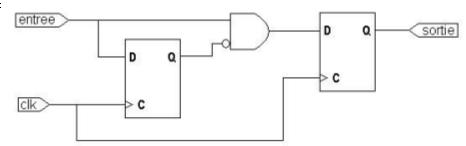
\includegraphics{I-circuit.png}

~

À l’arrivée du signal dans la porte logique, une entrée a été retardée plus ou moins aléatoirement, tandis que l’autre est directe. Il en résulte logiquement que le fonctionnement est aléatoire.

~

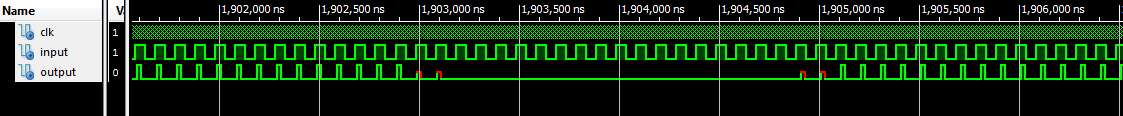
\includegraphics[width=\linewidth]{Setup_Hold_Post_Route.png}

~

À l’implémentation, il parait impossible de tomber sur un front non détecté à cause de ce problème. Cependant, en espaçant les bascules et donc en augmentant les temps de propagation, on observe sur l’oscilloscope (faute d’analyseur numérique…) très rapidement des fronts non détectés.

Pour corriger ce défaut, il faut synchroniser l’entrée non inverseuse de la porte logique en retardant son signal. Le meilleur moyen pour y arriver est d’utiliser le même composant (la bascule), pour assurer un retard semblable:

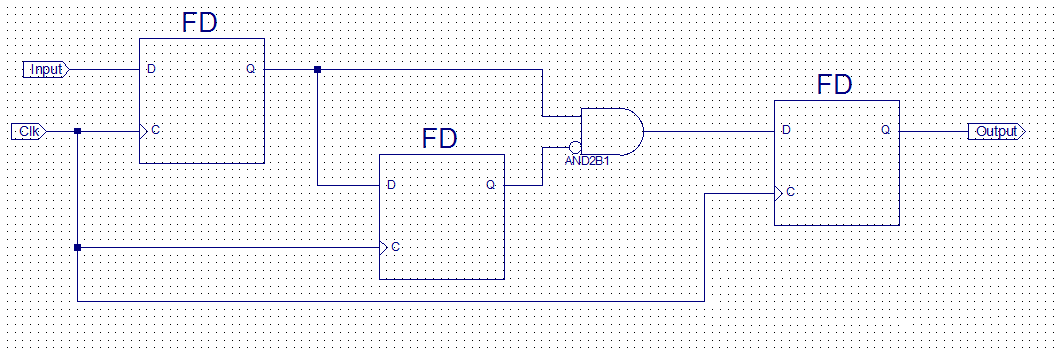
\includegraphics[width=\linewidth]{Setup_Hold_Synchronise.png}


On remarque donc que le problème a disparu sur la simulation.



Sur la carte de test, on n’observe plus de fronts non détectés, mais ça ne veut pas dire qu’il n’y en a plus.



On en déduit qu’il est impératif de synchroniser les signaux d’entrée avec la clk afin d’éviter des phénomènes dus aux temps de setup ou de hold non respectés.
\section{Réalisation d’une serrure codée}
\subsection{Conception asynchrone}

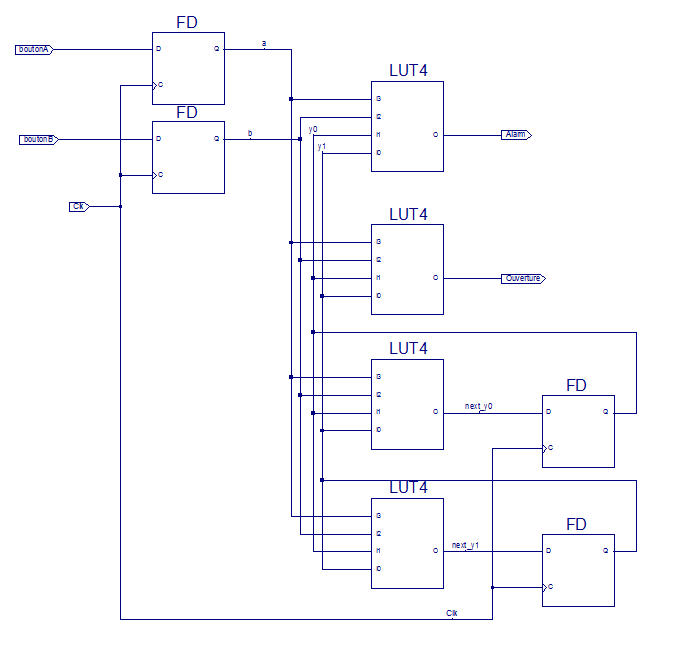
\includegraphics[width=\linewidth]{Serrure_Assynchrone.png}

\subsubsection{Étude de la fonction}

Après écriture d’un testbench où l’on fait varier les entrées de manière à suivre tous les chemins possible, on vérifie en simulation que les sorties correspondent au cahier des charges:

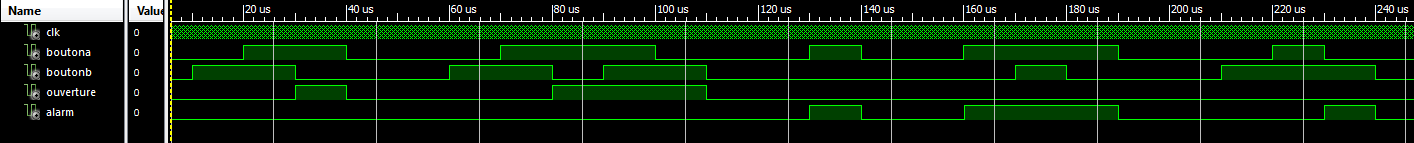
\includegraphics[width=\linewidth]{Serrure_Assynchrone_Testbench.png}


Cependant, après placement et routage, si l’on observe les signaux à l’intérieur des LUT, on observe des oscillations:

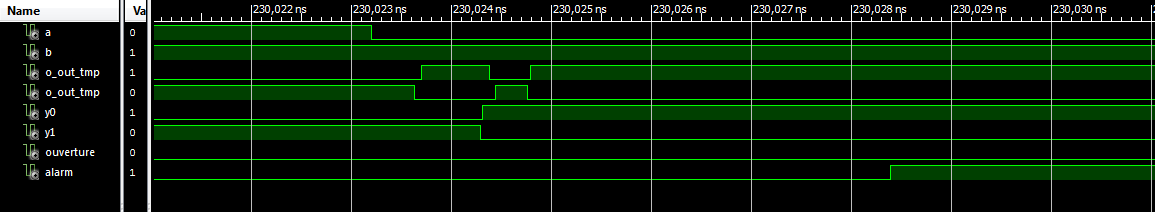
\includegraphics[width=\linewidth]{Serrure_Assynchrone_Oscillations.png}


Sur le passage de l’état «10» à l’état «01», les deux LUT s’inversent «en même temps», ce qui crée des phénomènes de cause critique.

Les paramètres qui influencent la période de ces oscillations sont les différences de délai sur les signaux d’entrée, et donc l’éloignement physique des différents composants sur le FPGA (placement/routage).
\subsubsection{Influence du routage}

En utilisant FloorPlan pour éclater le placement, puis en ajoutant des buffers également éclatés pour encore augmenter les temps de propagation, on n’observe pas spécialement d’effets sur les oscillations.



Cependant, dans le fichier \verb|timesim.sdf|, on voit bien que les temps de propagations sont très importants (plusieurs ns).
\subsection{Un parmi N}

Schématique générée à partir du VHDL:

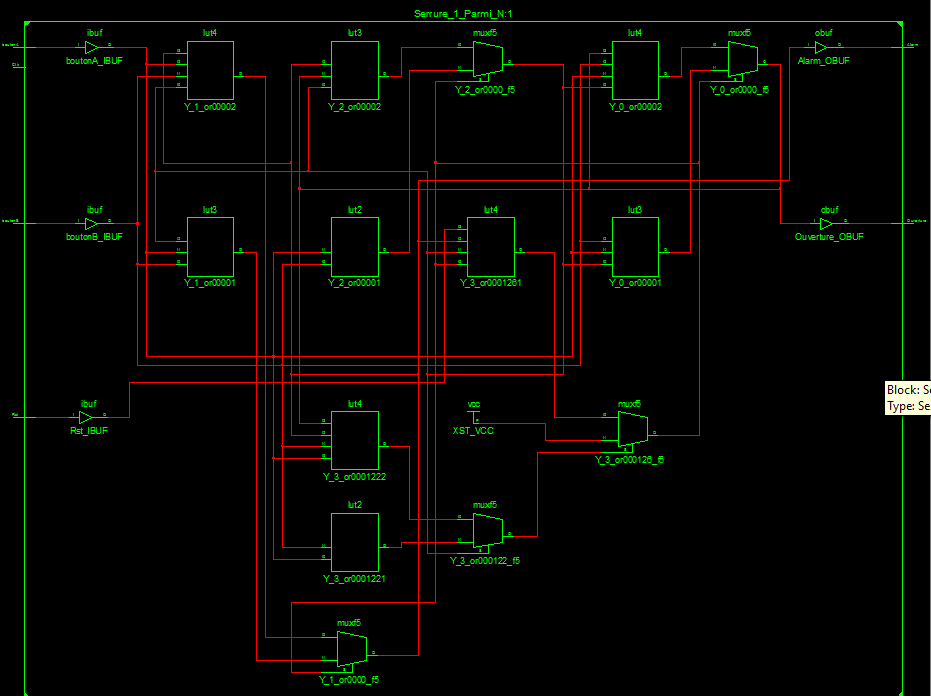
\includegraphics[width=\linewidth]{Serrure_1_Parmi_N_Sch.png}


On remarque que cette schématique est tout de même plus complexe que la précédente:

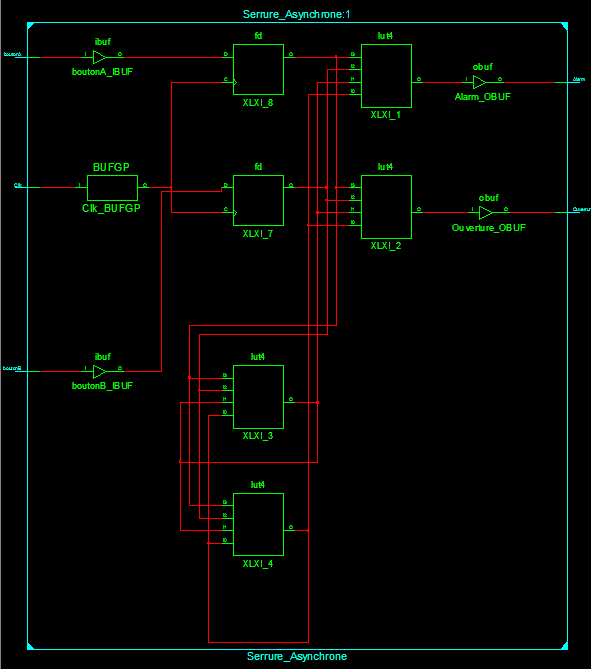
\includegraphics[width=\linewidth]{Serrure_Assynchrone_Sch.png}

\subsection{Conception synchrone}

Si l’on considère un conception synchrone seulement au niveau des entrées (boutons poussoirs), une modification simultanée des entrées peut avoir lieu, ce qui entraîne des cas indéterminés par rapport aux tables de vérité, et peut entrainer un comportement inatendu. Cette modification simultanée n’est possible que dans le mode de simulation «Behavioral», donc il n’est pas nécessaire de la prendre en compte (dans la vraie vie et dans les autres modes de simulation, les longueurs des pistes sont différentes, donc rien ne peut avoir lieu en même temps).

~

Cependant, ce système est plus robuste d’un point de vue des temps de propagation, car tant que les temps de propagation sont inférieurs à la période de CLK, on ne risque rien.

~

Maintenant, si on ajoute des bascules D sur les signaux Y, donc entre l’état courant et le calcul de l’état suivant, les problèmes rencontrés plus tôt disparaissent.
Il est donc intéressant de privilégier ce type de conception.


\end{document}
